%
% Niniejszy plik stanowi przykład formatowania pracy magisterskiej na
% Wydziale MIM UW.  Szkielet użytych poleceń można wykorzystywać do
% woli, np. formatujac wlasna prace.
%
% Zawartosc merytoryczna stanowi oryginalnosiagniecie
% naukowosciowe Marcina Wolinskiego.  Wszelkie prawa zastrzeżone.
%
% Copyright (c) 2001 by Marcin Woliński <M.Wolinski@gust.org.pl>
% Poprawki spowodowane zmianami przepisów - Marcin Szczuka, 1.10.2004
% Poprawki spowodowane zmianami przepisow i ujednolicenie 
% - Seweryn Karłowicz, 05.05.2006
% Dodanie wielu autorów i tłumaczenia na angielski - Kuba Pochrybniak, 29.11.2016

% dodaj opcję [licencjacka] dla pracy licencjackiej
% dodaj opcję [en] dla wersji angielskiej (mogą być obie: [licencjacka,en])
\makeatletter
\newenvironment{mcases}[1][l]
 {\let\@ifnextchar\new@ifnextchar
  \left\lbrace
  \def\arraystretch{1.2}%
  \array{@{}l@{\quad}#1@{}}}
 {\endarray\right.}
\makeatother

\documentclass[licencjacka]{pracamgr}
\usepackage[polish]{babel}
\usepackage{graphicx}
\usepackage{caption}
\usepackage{float}
\usepackage{subcaption}
\usepackage{amsmath}
\usepackage{algorithm2e}

% Dane magistranta:
\autor{Aleksander Mućk}{382184}


% Dane magistrantów:
%\autor{Aleksander Mućk}{342007}

\title{Algorytmy do klastrowania duplikacji genomowych}


\tytulang{Algorithms for the clustering of genomic duplications}

%kierunek: 
% - matematyka, informacyka, ...
% - Mathematics, Computer Science, ...
\kierunek{Bioinformatyka i Biologia Systemów}

% informatyka - nie okreslamy zakresu (opcja zakomentowana)
% matematyka - zakres moze pozostac nieokreslony,
% a jesli ma byc okreslony dla pracy mgr,
% to przyjmuje jedna z wartosci:
% {metod matematycznych w finansach}
% {metod matematycznych w ubezpieczeniach}
% {matematyki stosowanej}
% {nauczania matematyki}
% Dla pracy licencjackiej mamy natomiast
% mozliwosc wpisania takiej wartosci zakresu:
% {Jednoczesnych Studiow Ekonomiczno--Matematycznych}

% \zakres{Tu wpisac, jesli trzeba, jedna z opcji podanych wyzej}

% Praca wykonana pod kierunkiem:
% (podać tytuł/stopień imię i nazwisko opiekuna
% Instytut
% ew. Wydział ew. Uczelnia (jeżeli nie MIM UW))
\opiekun{dra hab. Pawła Góreckiego\\
  }

% miesiąc i~rok:
\date{Sierpień 2019}

%Podać dziedzinę wg klasyfikacji Socrates-Erasmus:
\dziedzina{ 
%11.0 Matematyka, Informatyka:\\ 
%11.1 Matematyka\\ 
%11.2 Statystyka\\ 
%11.3 Informatyka\\ 
%11.4 Sztuczna inteligencja\\ 
%11.5 Nauki aktuarialne\\
11.9 Inne nauki matematyczne i informatyczne
}

%Klasyfikacja tematyczna wedlug AMS (matematyka) lub ACM (informatyka)
\klasyfikacja{Computional biology, Applied computing, Life and medical sciences}

% Słowa kluczowe:
\keywords{duplikacja genu, drzewo genów, drzewo gatunków, analiza filogenetyczna, drzewo uzgadniające, Python, scenariusz ewolucyjny, strata genu, minimalizacja kosztu ewolucyjnego}

% Tu jest dobre miejsce na Twoje własne makra i~środowiska:
\newtheorem{defi}{Definicja}[section]

% koniec definicji

\begin{document}

\maketitle

%tu idzie streszczenie na strone poczatkowa

\begin{abstract}
   W niniejszej pracy przedstawione są propozycje algorytmów heurystycznych dla problemów klastrowania duplikacji genomowych w oparciu o scenariusze ewolucyjne. W części pierwszej wprowadzane są podstawowe pojęcia dotyczące drzew genów, gatunków, modeli ich uzgadniania oraz tworzenia scenariuszy ewolucyjnych. Omówiony został również problem przeliczania i klastrowania duplikacji genomowych. W części drugiej opisana została proponowana heurystyka wraz z przykładowymi testami oraz jej implementacją w języku Python.
\end{abstract}


\renewcommand{\contentsname}{Spis Treści}
\tableofcontents
%\listoffigures
%\listoftables

\chapter*{Wprowadzenie}
\addcontentsline{toc}{chapter}{Wprowadzenie}


Badanie drzew genów i gatunków, a w szczególności zależności między nimi może odpowiedzieć na pytania w jaki sposób wyodrębniały się gatunki przez pryzmat zmian w ich genomie. Mimo wszystko jednak należy pamiętać, że pokrewieństwo gatunków nie zawsze implikuje pokrewieństwo genów. W szczególności drzewo ewolucyjne genów nie musi pokrywać się z odpowiadającym im drzewem gatunków, które samo w sobie nie jest tak bardzo bardzo zróżnicowane jak drzewo genów. Tworzenie scenariuszy ewolucyjnych dzięki którym możemy poznać w jaki sposób ewolucja genów wpływała na ewolucję gatunków jest zadaniem nietrywialnym. Potrzebne są narzędzia, które potrafiłyby tworzyć i oceniać scenariusze pod kątem ilości zdarzeń ewolucyjnych i przyporządkować je we właściwe miejsca historii ewolucyjnej.

Wybranie właściwego scenariusza ewolucyjnego nie jest zadaniem łatwym, ponieważ takich scenariuszy, wyjaśniających ewolucję danej rodziny genów jest nieskończenie wiele. Problem jeszcze bardziej komplikuje się gdy w badaniach uwzględnimy wiele drzew genów, co generuje olbrzymią liczę danych do przeliczenia.

Należy pamiętać, że badacze nie zawsze maja dostęp do pełnych danych, a~i~te same w~sobie mogą być obarczone błędami. Do tego typu utrudnień należą między innymi: straty genów, braki w samych sekwencjach genomowych, czy niedokładne metody obliczania drzew genów i~gatunków, które są często niegwarantującymi optymalnych rozwiązań heurystykami. 

W niniejszej pracy proponowane są algorytmy heurystyczne, które oceniają zbiór scenariuszy tworząc na ich podstawie jeden, którego koszt, liczony jako liczba duplikacji, będzie możliwie najmniejszy.
\\
Praca składa się z~trzech rozdziałów i~dodatków.
Rozdział \ref{r:pojecia} zawiera podstawowe pojęcia dotyczące drzew genów, drzew gatunków oraz modeli i scenariuszy ewolucyjnych.  
Rozdział~\ref{r:heurystyka} przedstawia propozycję heurystyki wraz~z jej testami.  W~rozdziale tym opisano również implementację i sposób użycia programu napisanego na podstawie przedstawionej wcześniej heurystyki.
Ostatni rozdział zawiera przemyślenia dotyczące możliwego użycia algorytmu i~perspektyw jego rozwoju. W~dodatkach umieszczono fragmenty kodu i~przykładowe dane wejściowe.

\chapter{Podstawowe pojęcia}\label{r:pojecia}

W tym rozdziale poruszane są pojęcia i definicje niezbędne do zrozumienia problematyki klastrowania duplikacji genomowych. 
\section{Wstęp biologiczny}

Ewolucja biologiczna jest procesem zmian w trakcie których organizmy stopniowo nabywają lub tracą pewne cechy. Jest to element kluczowy dla powstawania nowych gatunków: specjacji. Śledzenie w jaki sposób kształtowały się nowe gatunki i w jaki sposób zachodziły na Ziemi procesy ewolucyjne jest zadaniem złożonym i wymagającym specyficznego podejścia. Jednym z możliwych sposobów przedstawienia historii ewolucyjnej gatunków jest drzewo filogenetyczne, które przedstawiają zależności ewolucyjne pomiędzy umieszczonymi na nim gatunkami lub genami. 

Początkowo za wyznacznik pokrewieństwa gatunków służyło podobieństwo morfologiczne, jednak jeśli dane molekularne są dostępne stosuje się metody polegające na badaniu podobieństwa danych rodzin genów. Można założyć, że im większe podobieństwo genów danych organizmów tym bliżej są one spokrewnione. Z punktu widzenia tej pracy genom jest niczym więcej jak zbiorem genów obecnym w danym organizmie. 


\section{Drzewa genów i gatunków}

W pracy tej drzewo to ukorzenione, binarne drzewo $T$ o zbiorze krawędzi skierowanych $E_T$~i zbiorze węzłów~$V_T$:
\begin{center}
T = $\langle V_T$ , $E_T  \rangle$,
\end{center}
%($v_1$ , $v_2$) takie, że $V_T$ \ni $v_x$ , $v_y$ .
gdzie $E_T$ zawiera pary węzłów ($v$,$w$) takie, że $v$,$w$ $\in$ $V_T$. Węzły z których nie wychodzą żadne krawędzie nazywane są liśćmi, a korzeń jest węzłem do którego nie prowadzą żadne krawędzie (nieposiadającym rodzica). Węzeł $v$ jest przodkiem węzła $w$ jeśli istnieje ścieżka skierowana z węzła $v$ do węzła $w$. Liczba krawędzi w ścieżce od węzła $v$ do węzła $w$ jest nazywana długością. Długość węzła $v$ od korzenia nazywana jest głębokością. Poddrzewem węzła $v$ jest drzewo oznaczone $T(v)$ w którym węzeł $v$ jest korzeniem. 
%Wszystkie etykiety obecne na liściach widoczne z wierzchołka $v_x$ oznaczmy jako L($v_x$).

Związki między gatunkami przedstawia się za pomocą drzewa~$T$, zwanego drzewem gatunków~S.
\begin{defi}\label{Drzewa gatunków}
  Drzewo gatunków to takie drzewo $S$, gdzie każdy liść reprezentuje gatunek, a~węzły wewnętrzne nazywamy specjacjami. Zbiór wszystkich gatunków (liści) w drzewie $S$ oznaczony jest jako $L(S)$. 
\end{defi}

Związki między genami w danej rodzinie przedstawia się za pomocą drzewa~T, zwanego drzewem genów~G.
\begin{defi}\label{Drzewa genów}
  Drzewo genów to takie drzewo $G$, gdzie każdy liść reprezentuje gen i jest etykietowony gatunkiem, z którego dany gen został zsekwencjonowany. Zbiór wszystkich gatunków (etykiet) w drzewie G oznaczony jest jako $L(G)$.
\end{defi}


\begin{figure}[H]
	\centering
	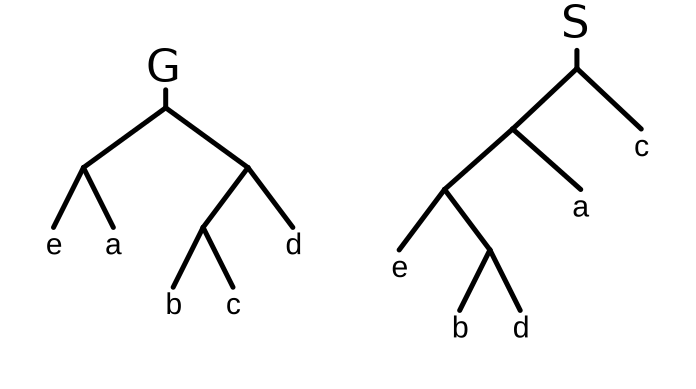
\includegraphics[width=100mm]{./pictures/spec_gen.png}
	\caption{Przykładowe drzewa genów $G$ i gatunków $S$ takie, że $L(G)=L(S)$ oraz~a,b,c,d~i~e~to~gatunki.}
\end{figure}

\section{Uzgodnienie drzew}
Bardzo częste różnice struktury drzewa genów w stosunku do historii ewolucyjnej opisanej drzewem gatunków wymagają mapowania węzłów drzewa $G$ na węzły znajdujące się w drzewie $S$. Jest to krok niezbędny by zrozumieć w jaki sposób ewolucja gatunków wpływała na strukturę ich genomów. 

\subsection{Mapowanie LCA}
Podstawowym algorytmem dla tego typu uzgodnień jest \textbf{algorytm LCA} (ang. \textit{Lowest Common Ancestor}; pl. \textit{Najniższy Wspólny Przodek}) \cite{PAGE:1994jv}. Najniższym przodkiem węzłów $v$ i $w$ to taki węzeł oznaczony jako $LCA(v,w)$, który jest przodkiem obu węzłów i którego długość ścieżki od korzenia drzewa jest największa. Najniższego wspólnego przodka dwóch węzłów można policzyć w czasie stały po liniowym, jednorazowym preprocesingu. 

\begin{defi}
Dla drzewa genów $G$ i drzewa gatunków $S$ takich, że $L(G)$ $\subseteq$ $L(S)$ mapowanie LCA to funkcja $MAP_{LCA}$: $V_G$ $\rightarrow$ $V_S$ gdzie dla każdego węzła $g$ z~drzewa genów $G$ $MAP_{LCA}$($V_G$) to węzeł taki, że:
\[ MAP_{LCA}(g) =
  \begin{cases}
    \text{etykieta }g       & \quad \text{jeśli } g \text{ jest liściem,}\\
    LCA(MAP_{LCA}(g_1),MAP_{LCA}(g_2))  & \quad \text{jeśli } g \text{ ma synów } g_1 \text{ i } g_2.
  \end{cases}
\]
\end{defi}

\begin{figure}[H]
  \centering
  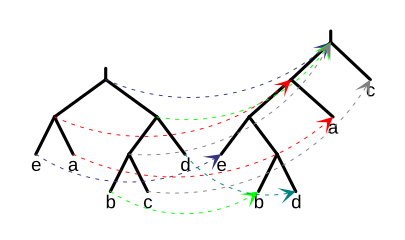
\includegraphics[width=80mm]{./pictures/mapping.png}
  \caption{Mapowanie $MAP_{LCA}$ dla przykładowego drzewa genów $G$ i gatunków $S$.}
\end{figure}

\subsection{Drzewa DLS}

Scenariusz ewolucyjny jest przedstawieniem ewolucji danej rodziny genów, przy uwzględnieniu ewolucji gatunków, które owe geny zawierają. Jako reprezentację scenariusza ewolucyjnego można stosować drzewa DLS (ang. \textit{Duplication-Loss-Speciation Tree}) \cite{Gorecki2006dls}. Drzewa te posiadają dwa rodzaje węzłów wewnętrznych i dwa rodzaje liści. Pierwszy rodzaj węzła wewnętrznego opisuje zjawisko duplikacji, czyli powielenia tego samego genu do dwóch kopii (oznaczmy jako DUP), zaś drugi jest wyrażeniem zjawiska specjacji (oznaczmy jako SPEC). Pierwszy z rodzajów liści jest opisuje stratę genu (oznaczmy jako LOSS), a drugi jest reprezentacją sekwencji genu obecnego w gatunku o danej etykiecie. Drzewo DLS w kontekście drzewa gatunków $S$ definiuje się w następujący sposób, gdzie $L(T)$ to zbiór wszystkich gatunków występujących w $T$:


\begin{enumerate}
\item $s$ jest drzewem DLS z jednym węzłem oznaczającym, że sekwencja genu jest obecna w gatunku $s$ i $L(s)=\{s\}$,
\item  A- jest drzewem DLS z jednym węzłem oznaczającym stratę genu, gdzie A jest niepustym zbiorem gatunków i $L(A-)=A$,
\item ($R_1$,$R_2$)+ jest drzewem DLS, którego korzeń jest węzłem duplikacyjnym i dzieci korzenia $R_1$ i $R_2$ są drzewami DLS takimi, że $L(R_1) = L(R_2)$,
\item ($R_1$,$R_2$)$\sim$ jest drzewem DLS, którego korzeń jest węzłem specjacyjnym i dzieci korzenia $R_1$ i $R_2$ są drzewami DLS takimi, że $L(R_1) \cap L(R_2) = 0$.
\end{enumerate}

Z każdego drzewa DLS możliwe jest odczytanie drzewa genów. Operację tę oznaczoną jako $gene(T)$, gdzie $T$ jest drzewem DLS definiuje się w następujący sposób \cite{Gorecki2006dls}:
\begin{enumerate}
\item $gene(\emptyset)=\emptyset$,
\item $gene(s)=s$ ,
\item $gene(A-)=\emptyset$,
\item Dla $\star \in \{\sim , + \}$: 
\begin{equation*} 
gene((R_2,R_2)\star)=
  \begin{mcases}[ll@{\ }l]
  \emptyset              & \text{jeśli } gene(R_1)= \emptyset =gene(R_2),\\
  gene(R_1)              & \text{jeśli } gene(R_1) \neq \emptyset =gene(R_2),\\
  gene(R_2)              & \text{jeśli } gene(R_1)= \emptyset \neq gene(R_2),\\
  (gene(R_2),gene(R_2))  & \text{w innym przypadku. } \\
\end{mcases}
\end{equation*}
\end{enumerate}

Klasyczną miarą kosztu ewolucyjnego danego drzewa DLS jest liczba znajdujących się w nim węzłów duplikacyjnych. Dla przykładu koszt ten dla drzewa DLS widocznego na rysunku 1.3 wynosi 1, ponieważ znajduje się w nim tylko jeden węzeł duplikacyjny.

\subsection{Scenariusz LCA}

Z wykorzystaniem mapowania LCA węzłów drzewa genów $G$ do drzewa gatunków $S$ można stworzyć drzewo DLS, które reprezentuje scenariusz LCA.

\begin{defi}
Scenariusz LCA dla drzewa $G$ o korzeniu $g$ i drzewa $S$ o korzeniu $s$, gdzie $L(G) \subseteq L(S)$, jest drzewem DLS $p(g,MAP_{LCA}(g))$, takim, że $p(g,s)$ = $s$ kiedy $g$ i $s$ są liśćmi oraz etykietą $g$ jest $s$. W innym przypadku:

\begin{equation*} 
p(g,s) =
  \begin{mcases}[ll@{\ }l]
  (p(g,u),L(T(v))-)\sim  & \text{jeśli } MAP_{LCA}(g) \in T(u), & (LOSS)\\
  (p(q,u),p(r,v))\sim    & \text{jeśli } MAP_{LCA}(q) \in T(u)\wedge MAP_{LCA}(r) \in T(v), & (SPEC)\\
  (p(q,s),p(r,s))+       & \text{jeśli } MAP_{LCA}(g) = MAP_{LCA}(q) = s, & (DUP)
\end{mcases}
\end{equation*}
gdzie \textit{u} oraz \textit{v} są dziećmi \textit{s}, a dzieci \textit{g} to \textit{q} oraz \textit{r}. 
\end{defi}

\begin{figure}[H]
  \centering
  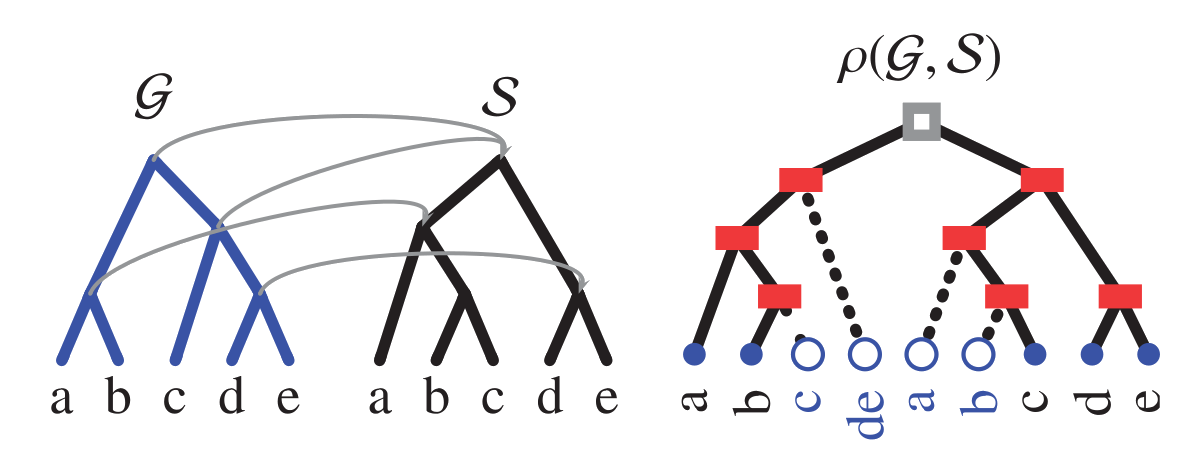
\includegraphics[width=120mm]{./pictures/DLS.png}
  \caption{Drzewo DLS $p(G,S)$ będące scenariuszem zbudowanym w oparciu o mapowanie LCA, które uzgadnia drzewo genów $G$ i drzewo gatunków $S$. Węzeł oznaczony szarym kwadratem jest węzłem duplikacyjnym, a czerwony prostokąt jest specjacją. Gałęzie narysowane linią przerywaną prowadzą do liści, które są reprezentacją straty genów w danym gatunku. Rysunek pochodzi z pracy \cite{Gorecki2006dls}.}
\end{figure}

Przedstawieniem drzewa DLS jest "wbudowanie" drzewa genów, w kontener będący drzewem gatunków. 


\begin{figure}[H]
  \centering
  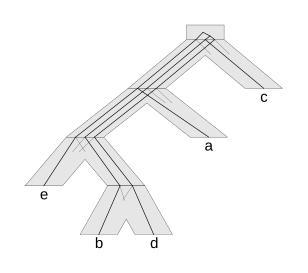
\includegraphics[width=80mm]{./pictures/optscen.png}
  \caption{Przykład wbudowania dla drzew z rysunku 1.2.}
\end{figure}

\section{Klastrowanie duplikacji}

Jednym z problemów podczas tworzenia scenariuszy ewolucyjnych jest problem jednoczesnych duplikacji genomowych. Istnieje potrzeba wprowadzenia dodatkowych reguł, które określą, kiedy dwie duplikacje mogą być klastrowane razem. 
 
Niech $S$ to drzewo gatunków z~węzłami $\langle s_1,s_2, \dots , s_m \rangle$.
Niech $\mathcal{T}=\{T_1,T_2, \dots , T_n\}$ to drzewa DLS takie, że $L(gene(T_i)) \subseteq L(S)$ dla każdego $i$ oraz $T_i$ jest wektorem $\langle e^1,e^2, \dots , e^m \rangle$, gdzie dla każdego $j$, $e^j$ to liczba epizodów duplikacyjnych przypisanych do węzła $s_j$. Wówczas mówimy, że dwa węzły duplikacyjne $d_1$ i $d_2$ z $\mathcal{T}$ można sklastrować (oznaczymy jako $d_1$~$\Longleftrightarrow$~$d_2$)  jeśli poniższe warunki są spełnione:
\begin{itemize}
\item $L(d_1) = L({d_2})$,
\item jeśli $d_1$ i $d_2$ są w jednym drzewie DLS to nie leżą na jednej ścieżce (są nieporównywalne) albo $d_1=d_2$.
\end{itemize}

Klastrowanie opisane powyżej to klastrowanie ME (ang. \textit{Minimum Episodes Clustering}) i zostało po raz pierwszy zaproponowane w pracy \cite{Guigo1996}. Będzie ono również używane w tej pracy.

\begin{defi}\label{MEs}
  MEScore($\mathcal{T}, S, j) = \min_{\cup P = {Dup}_s(\mathcal{T},j)} \lbrace \vert P \vert\ : \forall_{A \in P} \forall_{d_1,d_2 \in A} d_1 \Longleftrightarrow d_2 \rbrace$
 gdzie ${Dup}_s(\mathcal{T},j$) jest zbiorem wszystkich węzłów duplikacyjnych obecnych w $\mathcal{T}$, których klaster jest równy $L(s_j)$. 
\end{defi}


MEScore($\mathcal{T}$, $S$) to wtedy minimalna wielkość podziału zbioru wszystkich węzłów duplikacyjnych obecnych w scenariuszach tak, że każde dwie duplikacje z tego samego podziału są klastrowalne. Formalnie:

\begin{defi}\label{ME}
  MEScore($\mathcal{T}$, $S$) = $\sum_{j \in \{1,\dots,m\}} MEScore(\mathcal{T}, S, j)$.
\end{defi}

\begin{figure}[H]
  \centering
  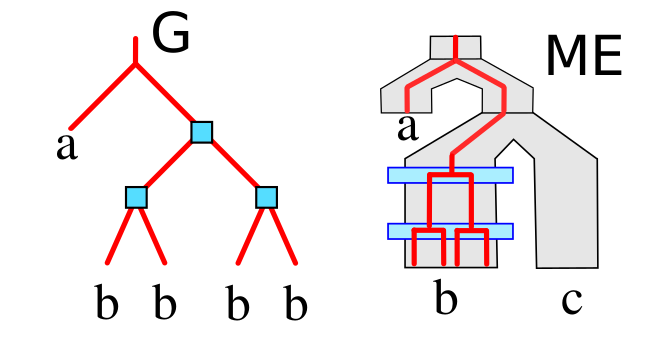
\includegraphics[width=70mm]{./pictures/clas_type_me.png}
  \caption{Klastrowanie ME dla przykładowego drzewa genów $G$. Rysunek zaadaptowany z pracy \cite{RME}.}
\end{figure}


Klastrowanie ME nie jest jedynym możliwym rodzajem klastrowania. Wyróżnia się także klastrowania:
\begin{itemize}
\item GD, gdzie duplikacje nie mogą zostać sklastrowane jeśli obecne są w tym samym drzewie DLS.
\item EC, gdzie duplikacje mogą zostać sklastrowane jeśli węzły duplikacyjne mapują do tego samego węzła na drzewie gatunków.
\end{itemize}
~\linebreak
Definicje na podstawie pracy \cite{RME}.

\section{Modele scenariuszy ewolucyjnych}

Drzewo DLS, które opiera się o mapowanie LCA, jest drzewem o możliwie najmniejszym koszcie duplikacyjnym i możliwe najgłębiej położonych węzłach duplikacyjnych. Nie jest to jednak jedyny możliwy scenariusz, których w rzeczywistości jest nieskończenie wiele. Należy jednak pamiętać, że nie powinno się brać pod uwagę przypadków skrajnie nieprawdopodobnych, gdzie gen jest, dla przykładu, wielokrotnie duplikowany i tracony. Po wprowadzeniu tego typu ograniczeń możliwe jest otrzymanie skończonego zbioru możliwych scenariuszy ewolucyjnych, które zwane są semi-normalnymi. Formalnie drzewo DLS nazywamy semi-normalnym jeśli:
\begin{itemize}
\item nie istnieje węzeł duplikacyjny, którego dzieckiem jest strata,
\item nie istnieje węzeł specjacyjny, którego dzieci są stratami.
\end{itemize}


\subsection{Transformacje scenariuszy ewolucyjnych}

Drzewo DLS podlega ściśle określonym transformacjom, które zmieniają jego strukturę: 
\begin{enumerate}
\item TMOVE: Poddrzewo $((C-,P)\sim,(C-,Q)\sim))+$ w drzewie DLS zostaje zamienione na poddrzewo $(C-,(P,Q)+)\sim $ ,
\item CLOST: Poddrzewo $((P,L(Q)-)\sim,(L(P)-,Q)\sim)+$ w drzewie DLS zostaje zamienione na poddrzewo $(P,Q)\sim $ ,
\end{enumerate}
gdzie $C,P,Q$ są drzewami DLS.

\begin{figure}[H]
  \centering
  \includegraphics[width=120mm]{./pictures/move.png}
  \caption{Transformacje TMOVE i CLOST wraz z ich biologiczną interpretacją. Szary  kwadrat reprezentuje duplikację. Czerwony prostokąt i czerwona linia przerywana są reprezentacją specjacji, a niebieskie koło jest stratą. Rysunek zaadaptowany z pracy \cite{Gorecki2006dls}.}
\end{figure}



Stosowane są również odwrotności zdefiniowanych powyżej transformacji, które oznaczone są indeksem górnym~$^{-1}$ np. TMOVE$^{-1}$.

Dla ustalonego drzewa genów $G$ i ustalonego drzewa gatunków $S$, gdzie $L(G) \subseteq L(S)$, możliwe jest uzyskanie zbioru scenariuszy semi-normalnych, który reprezentowany jest jako zbiór drzew DLS, poprzez zastosowanie ruchów TMOVE$^{-1}$ i CLOST$^{-1}$ na drzewie DLS będącym scenariuszem LCA. 

Na rysunku 1.7 przedstawione są wszystkie możliwe przekształcenia TMOVE i CLOST dla przykładowych drzew $G$ i $S$.

\subsection{Opis modeli dopuszczalnych scenariuszy}

W praktyce nie zawsze rozważa się wszystkich możliwych scenariuszy do klastrowania, ponieważ może prowadzić to do nieprawdopodobnych klastrowań duplikacji np. gdzie wszystkie duplikacje ulokowane zostały w korzeniu drzewa DLS. Należy wspomnieć, że w przypadku straty genów duplikacje genomowe będą zazwyczaj położone niżej na drzewie gatunków. W niektórych sytuacjach może to wymusić użycie modeli, które pozwalają na wielokrotne transformacje drzew DLS i odejście od scenariusza LCA. Nie możliwe jest jednak dowolne przesuwanie węzła duplikacyjnego, ponieważ specjacja jest górnym ograniczeniem przy przesuwaniu duplikacji.

W literaturze wyodrębniono kilka dopuszczalnych modeli, a w pracy tej zajęto się podanymi niżej modelami, które dopuszczają podane warunki:
\begin{enumerate}
\item Model PG \cite{pg_EC2016}: Model ten dopuszcza tylko takie drzewa DLS, które zachowują minimalny koszt duplikacyjny. Oznacza to, że są to scenariusze osiągalne ze scenariusza LCA reprezentowanego drzewem DLS za pomocą transformacji TMOVE$^{-1}$.
\item Model FHS \cite{Fellows:1998:MGD}: Model ten dopuszcza każde możliwe przekształcenie drzew DLS, nawet jeśli takie drzewo nie zachowuje minimalnego kosztu duplikacyjnego. Oznacza to, że są to scenariusze osiągalne ze scenariusza LCA reprezentowanego drzewem DLS za pomocą transformacji TMOVE$^{-1}$ i CLOST$^{-1}$.
\end{enumerate}

Należy wspomnieć, że w przypadku straty genów duplikacje genomowe będą położone niżej na drzewie gatunków. Nie zawsze istnieje możliwość ich przesunięcia w dowolne miejsce, ponieważ specjacja jest górnym ograniczeniem przy przesuwaniu węzłów duplikacyjnych. Taka transformacja przekształciłaby scenariusz tak, że nie byłby on semi-normalny.

\section{Minimalizacja epizodów duplikacji}

Badania wielokrotnych duplikacji tworzą szeroką gamę problemów różniących się właściwościami, które zależą od metody klastrowania i modelu dozwolonych scenariuszy. W pracy tej zajęto się tylko klastrowaniem ME, więc problem minimalizacji epizodów jest parametryzowany wyłącznie przez obrany model scenariuszy. 

\newtheorem{problem}{Problem}
\begin{problem}
  Dane: drzewo gatunków $S$, zbiór drzew genów $\mathcal{G}=\{G_1,G_2, \dots , G_n\}$ gdzie dla każdego $i$ $L(G_i) \subseteq L(S)$ oraz $\mathcal{M}(G_i,S)$ jest zbiorem dopuszczalnych DLS drzew $T$ dla $G_i$ w~modelu $\mathcal{M}$ takich, że $gene(T)=G_i$. Znajdź scenariusz ewolucyjny, który minimalizuje liczbę epizodów duplikacji, oznaczoną jako RME i zdefiniowaną w następujący sposób:
  ${RME}_{\mathcal{M}}(\mathcal{G}, S) = \min_{\forall_i T_i \in \mathcal{M}(G_i,S)}MEScore(\lbrace T_i \rbrace_{i=1,2,\dots,n},S)$.
\end{problem}

Po raz pierwszy problem minimalizacji epizodów został opisany w pracy \cite{Guigo1996}.

\begin{figure}[t]\label{diagram_red}
  \centering
  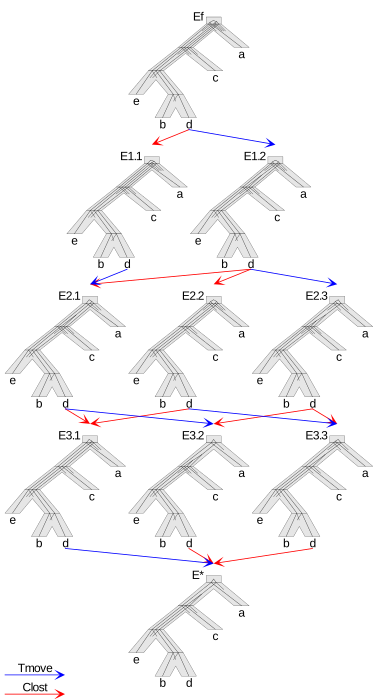
\includegraphics[height=200mm,keepaspectratio]{./pictures/diagram_2.png}
  \caption{Diagram przekształceń scenariuszy semi-normalnych. Na dole rysunku, oznaczone filetowym kołem, znajduje się drzewo uzyskane za pomocą mapowania LCA. Model PG zawierać będzie tylko drzewa oznaczone zielonym kołem, podczas gdy dla modelu FHS wszystkie drzewa obecne na diagramie są częścią zboru scenariuszy semi-normalnych.}
\end{figure}


\chapter{Algorytm do klastrowania duplikacji}\label{r:heurystyka}
Dane empiryczne wskazują, że klastrowanie duplikacji dla modelu PG i jego pochodnych jest zbliżone do tego wyznaczonego przez mapowanie LCA. Z tego powodu należałoby przeanalizować scenariusze wygenerowane z użyciem modeli bardziej ogólnych, takich jak model FHS. W tym rozdziale przedstawiony zostanie algorytm heurystyczny, który umożliwia uniwersalne klastrowanie duplikacji w modelach ogólniejszych niż model PG i w innych, które się o niego opierają.
\section{Opis algorytmu}
\begin{algorithm}[H]
 \KwIn{
 \begin{enumerate}
 \itemsep0em 
\item Drzewo gatunków $S$ z~węzłami $\langle s_1,s_2, \dots , s_m \rangle$,
\item Zbiór drzew genów $\mathcal{G}=\{G_1,G_2, \dots , G_n\}$ gdzie $L(G_i) \subseteq L(S)$ dla każdego $i$,
\item Zbiór drzew DLS $\mathcal{T}_i=\{T_i^1,T_i^2, \dots , T_i^{h_i}\}$ dla każdego drzewa genów $G_i \in \mathcal{G}$, reprezentowanych jako wektory  epizodów $\langle e^1_{i,j},e^2_{i,j}, \dots , e^m_{i,j} \rangle$, gdzie dla każdego $k$, $e^k_{i,j}$ to liczba epizodów duplikacyjnych przypisanych do węzła $s_k$ w $j$-tym drzewie DLS dla $i$-tego drzewa genów.
\end{enumerate}}
 \KwOut{Scenariusz w postaci wektora epizodów $\langle {e}^1,{e}^2, ... , {e}^m \rangle$.}
 $V^{max}$ := $\langle {e}^1,{e}^2, \dots , {e}^m \rangle$, gdzie dla każdego $k$, ${e}^k$=$max_{\forall_{i \in \{1,\dots,n\}},\forall_{j \in \{1,\dots,h_i\}}}e^k_{i,j}$\;
 $V^*$ := $V^{max}$\;
 \textbackslash\textbackslash \textit{Pętla główna}\;
 \For{k $\in \{1,\dots,m\}$}{
  $V_{new}^*$ = $V^*$\;
  zmiana := True\;
  \While{zmiana i ${V_{new}}^*[k] > 0$}{
  $V_{new}^*$[$k$] - -\;
  zmiana := False\;
  \If{$ \forall_{G_i \in \mathcal{G}}V_{new}^* \triangleright \mathcal{T}_i$}{
   \textbackslash\textbackslash \textit{Wyjaśnienie symbolu $\triangleright$ znajduje się pod algorytmem}\;
   $V^*$ := $V_{new}^*$\;
   zmiana := True\;
   }
   }
 }
\end{algorithm}


Niech $R$ będzie scenariuszem, a $\langle r^1,r^2, \dots , r^m \rangle$ wektorem epizodów, takim, że dla każdego $j$, $r^j$ to liczba epizodów duplikacyjnych w $R$ przypisanych do węzła $s_j$. Mówimy, że $R$ zawiera się w zbiorze scenariuszy $\mathcal{T}$ (oznaczone jako $R \triangleright \mathcal{T}$) jeśli: istnieje scenariusz ${T \in \mathcal{T}}$ taki, że $\forall_{j \in \{1,\dots,m\}}MEScore(\{T\},S,j) \geq r^j$.
\\
~\\
Wybór współrzędnej $k$ odpowiadającej pozycji węzła $s_k$ w pętli głównej może, zależnie od potrzeby, być dokonywany w inny sposób (np. w porządku prefiksowym) jednak w tej pracy współrzędne wybierane były losowo. Pętlę główną wykonywano dziesięć razy i uwzględniano najlepszy wynik. 

\section{Dokumentacja użytkowa i~opis implementacji}\label{r:impl}
Opisana heurystyka zaimplementowana została w języku Python w wersji 3.7.4 przy użyciu paradygmatu obiektowego, gdzie zbiór wszystkich drzew DLS dla wszystkich drzew, zbiór drzew semi-normalnych otrzymanych z jednego drzewa genów, a także pojedyncze drzewo DLS stanowią oddzielne klasy. Fragment kodu można zobaczyć w dodatku A. Program pythonowy przyjmuje na wejściu listę plików w których zawarte są wyliczone scenariusze dla danego drzewa genów.

Algorytm ten, dla wygody użycia, został obudowany skryptem napisanym w języku bash, który pozwala na wyliczenie scenariuszy w modelu FHS i PG z wykorzystaniem programu DLSgen autorstwa dra hab. Pawła Góreckiego. Program ten wylicza dla danego drzewa genów i drzewa gatunków scenariusze ewolucyjne, które wykorzystywane są jako dane wejściowe dla proponowanej heurystyki. Nie jest on jeszcze opublikowany i został wykorzystany za zgodą jego autora.


\section{Testy algorytmu}
Do sprawdzenia wyników wyliczanych przez proponowany algorytm użyty został program RME napisany przez dra Jarosława Paszka. Program ten korzystając z dostępnych metod algorytmicznych wylicza dokładne i najniższe możliwe wartości kosztu ewolucyjnego dla podanych modeli z użyciem klastrowania ME \cite{RME}.
\\
Z powodu trudności w obliczeniu danych wejściowych dla heurystyki obecnie nie ma możliwości przetestowania heurystyki dla dużych zbiorów danych.

\subsection{Testy algorytmu na danych rzeczywistych}
Zbiorem danych dla testu na danych rzeczywistych był zbiór Guigo zawierający 53 ukorzenione drzewa genów pochodzące od 16 eukariontów. Do zbioru tego załączono dwa drzewa gatunków $S_1$ z pracy \cite{Guigo1996} i $S_2$ z pracy \cite{Page1997RTI}. 

\begin{figure}[H]
\centering
\begin{subfigure}{.5\textwidth}
  \centering
  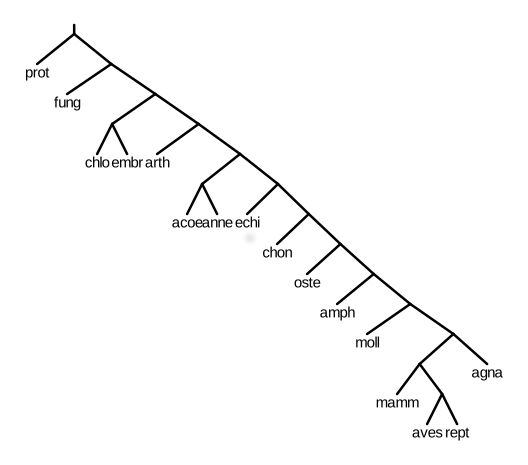
\includegraphics[width=50mm]{./pictures/guigo_spec_1.png}
  \caption{Drzewo $S_1$}
\end{subfigure}%
\begin{subfigure}{.5\textwidth}
  \centering
  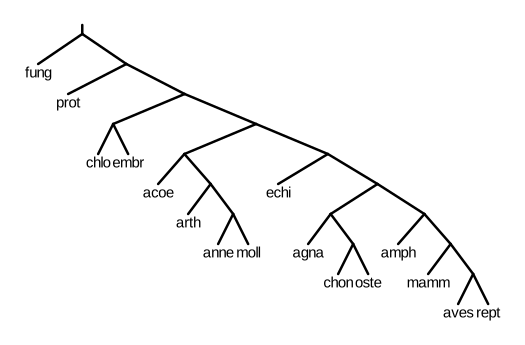
\includegraphics[width=50mm]{./pictures/guigo_spec_2.png}
  \caption{Drzewo $S_2$}
\end{subfigure}%
\caption{Drzewa gatunków ze zbioru Guigo}
\end{figure}

\begin{figure}[H]
\centering
\begin{subfigure}{.5\textwidth}
  \centering
  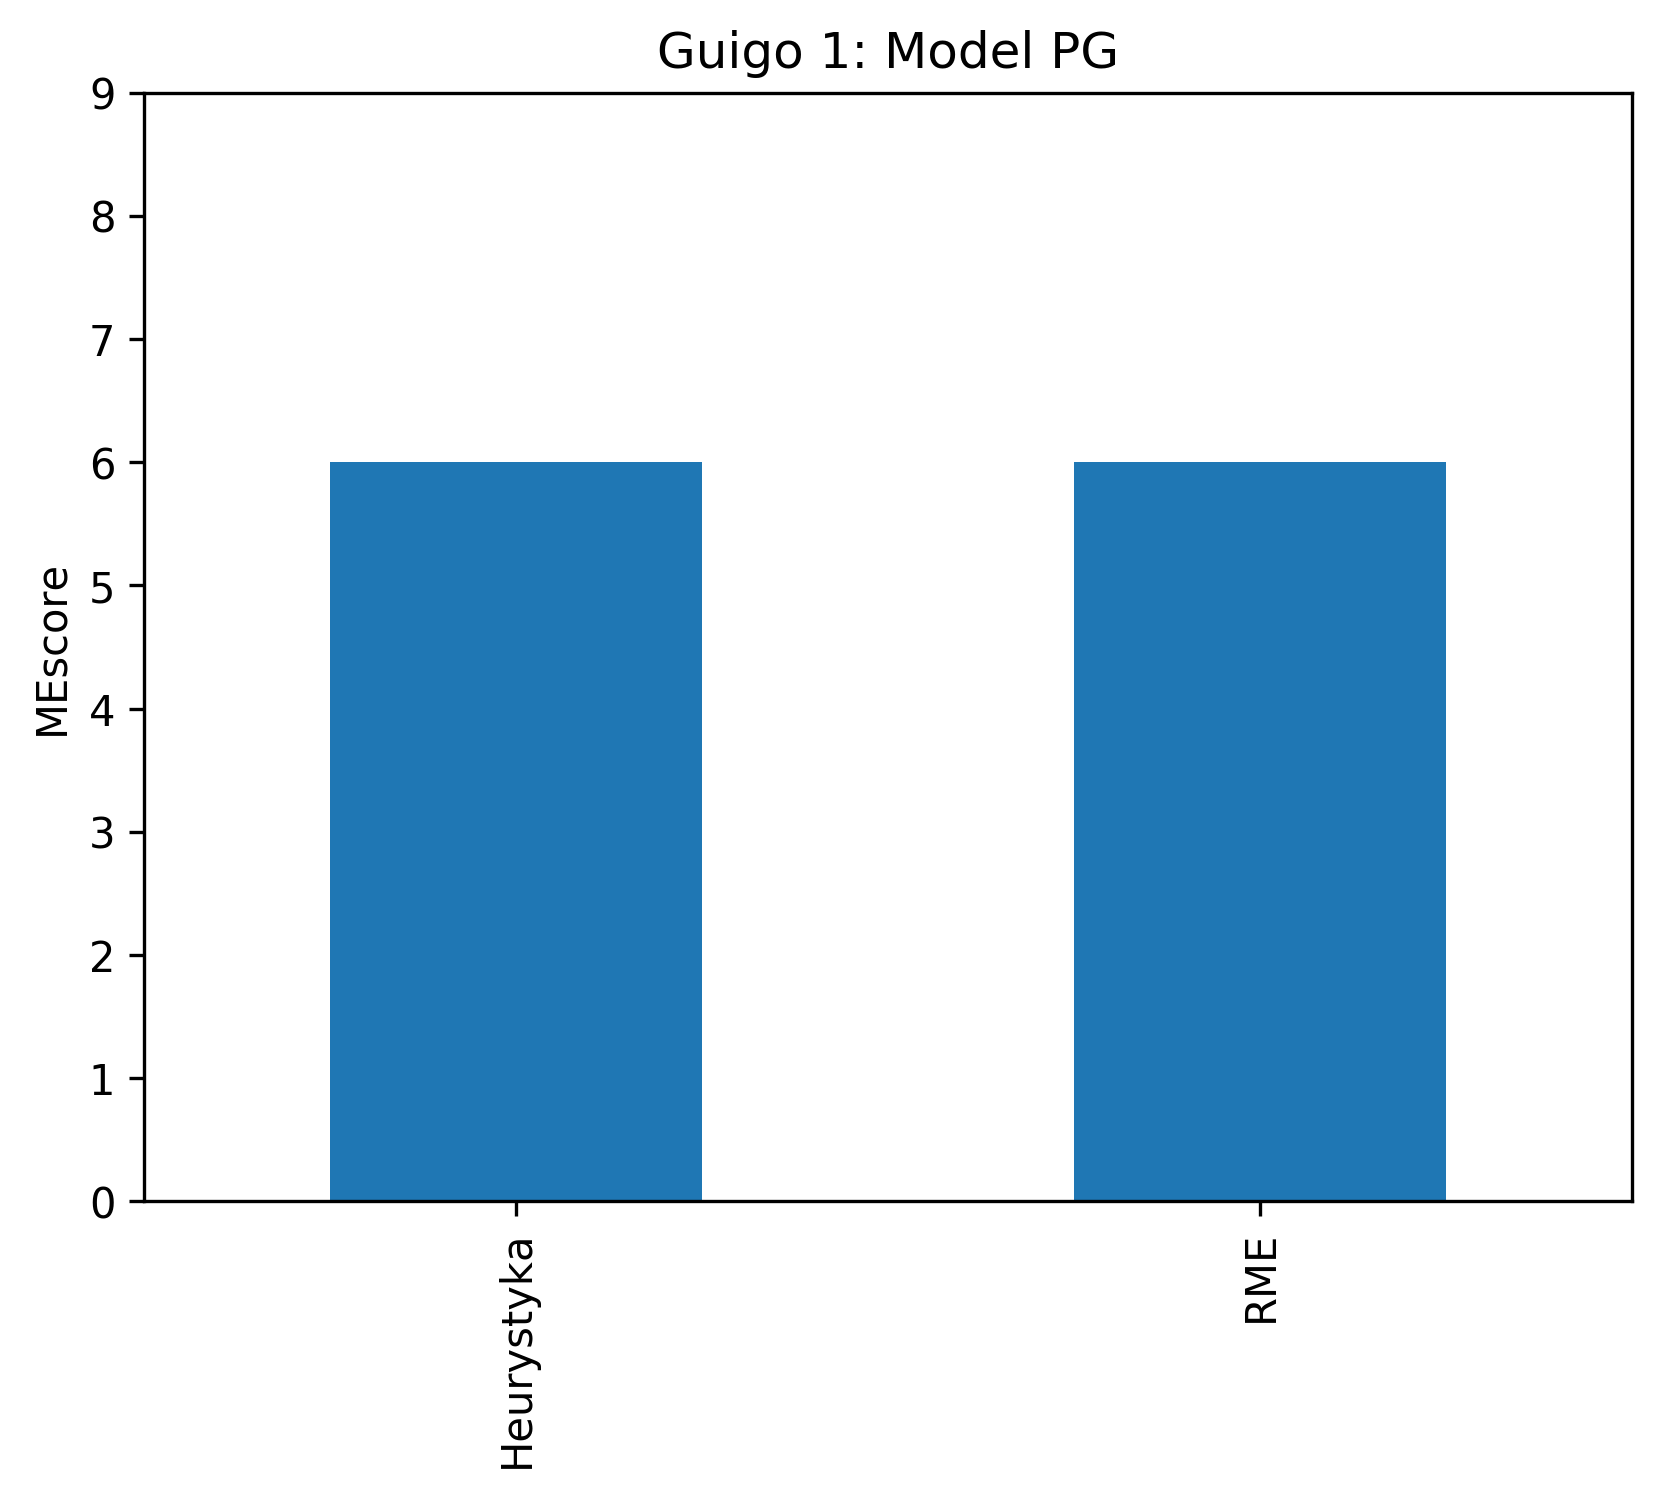
\includegraphics[width=50mm]{./pictures/G1_PG.png}
  \caption{Test algorytmu dla modelu PG}
\end{subfigure}%
\begin{subfigure}{.5\textwidth}
  \centering
  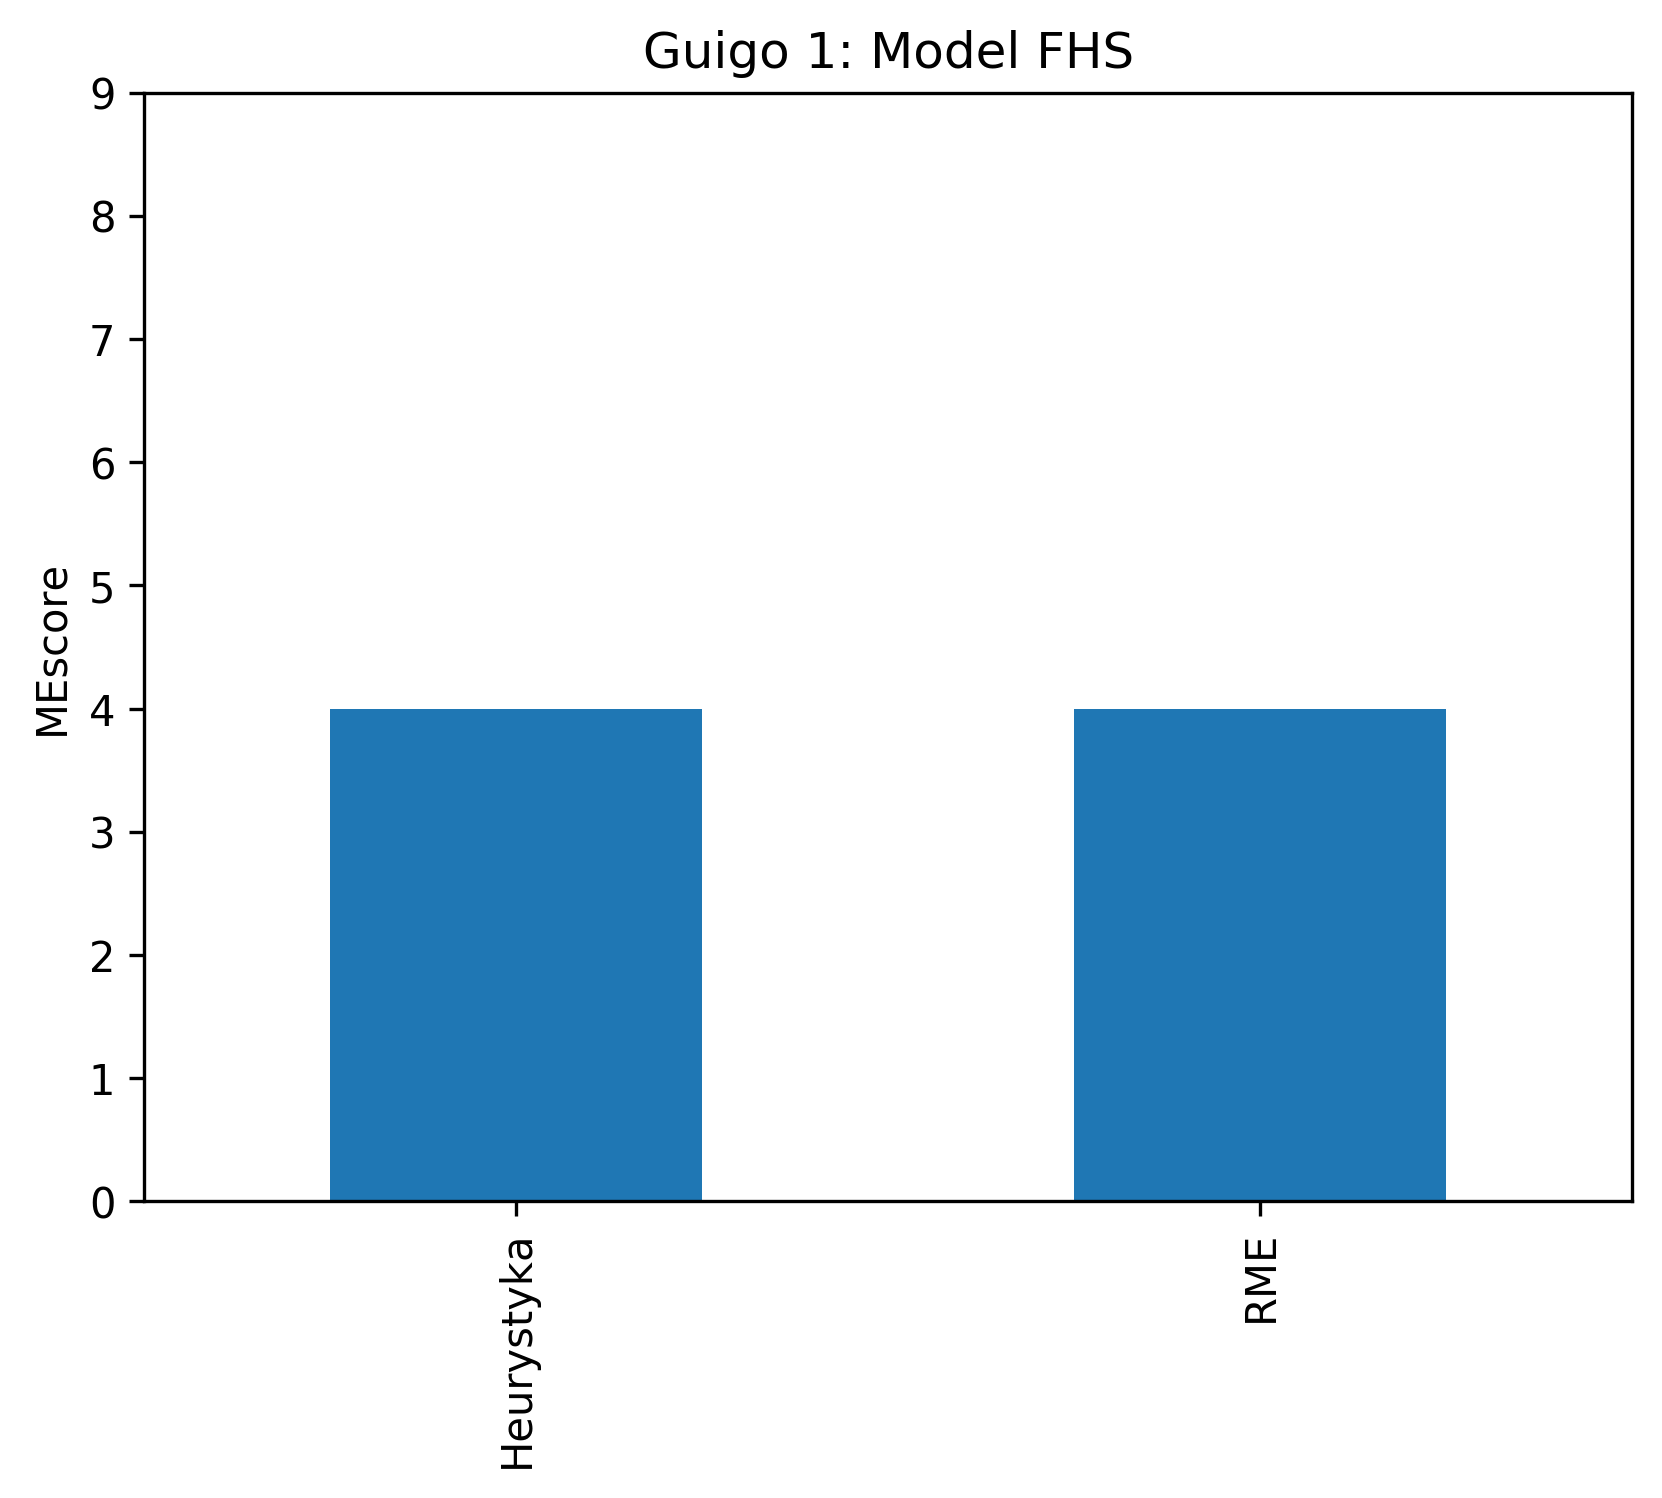
\includegraphics[width=50mm]{./pictures/G1_FHS.png}
  \caption{Test algorytmu dla modelu FHS}
\end{subfigure}%
\caption{Testy algorytmu na danych rzeczywistych dla drzewa gatunków $S_1$}
\end{figure}


\begin{figure}[H]
\centering
\begin{subfigure}{.5\textwidth}
  \centering
  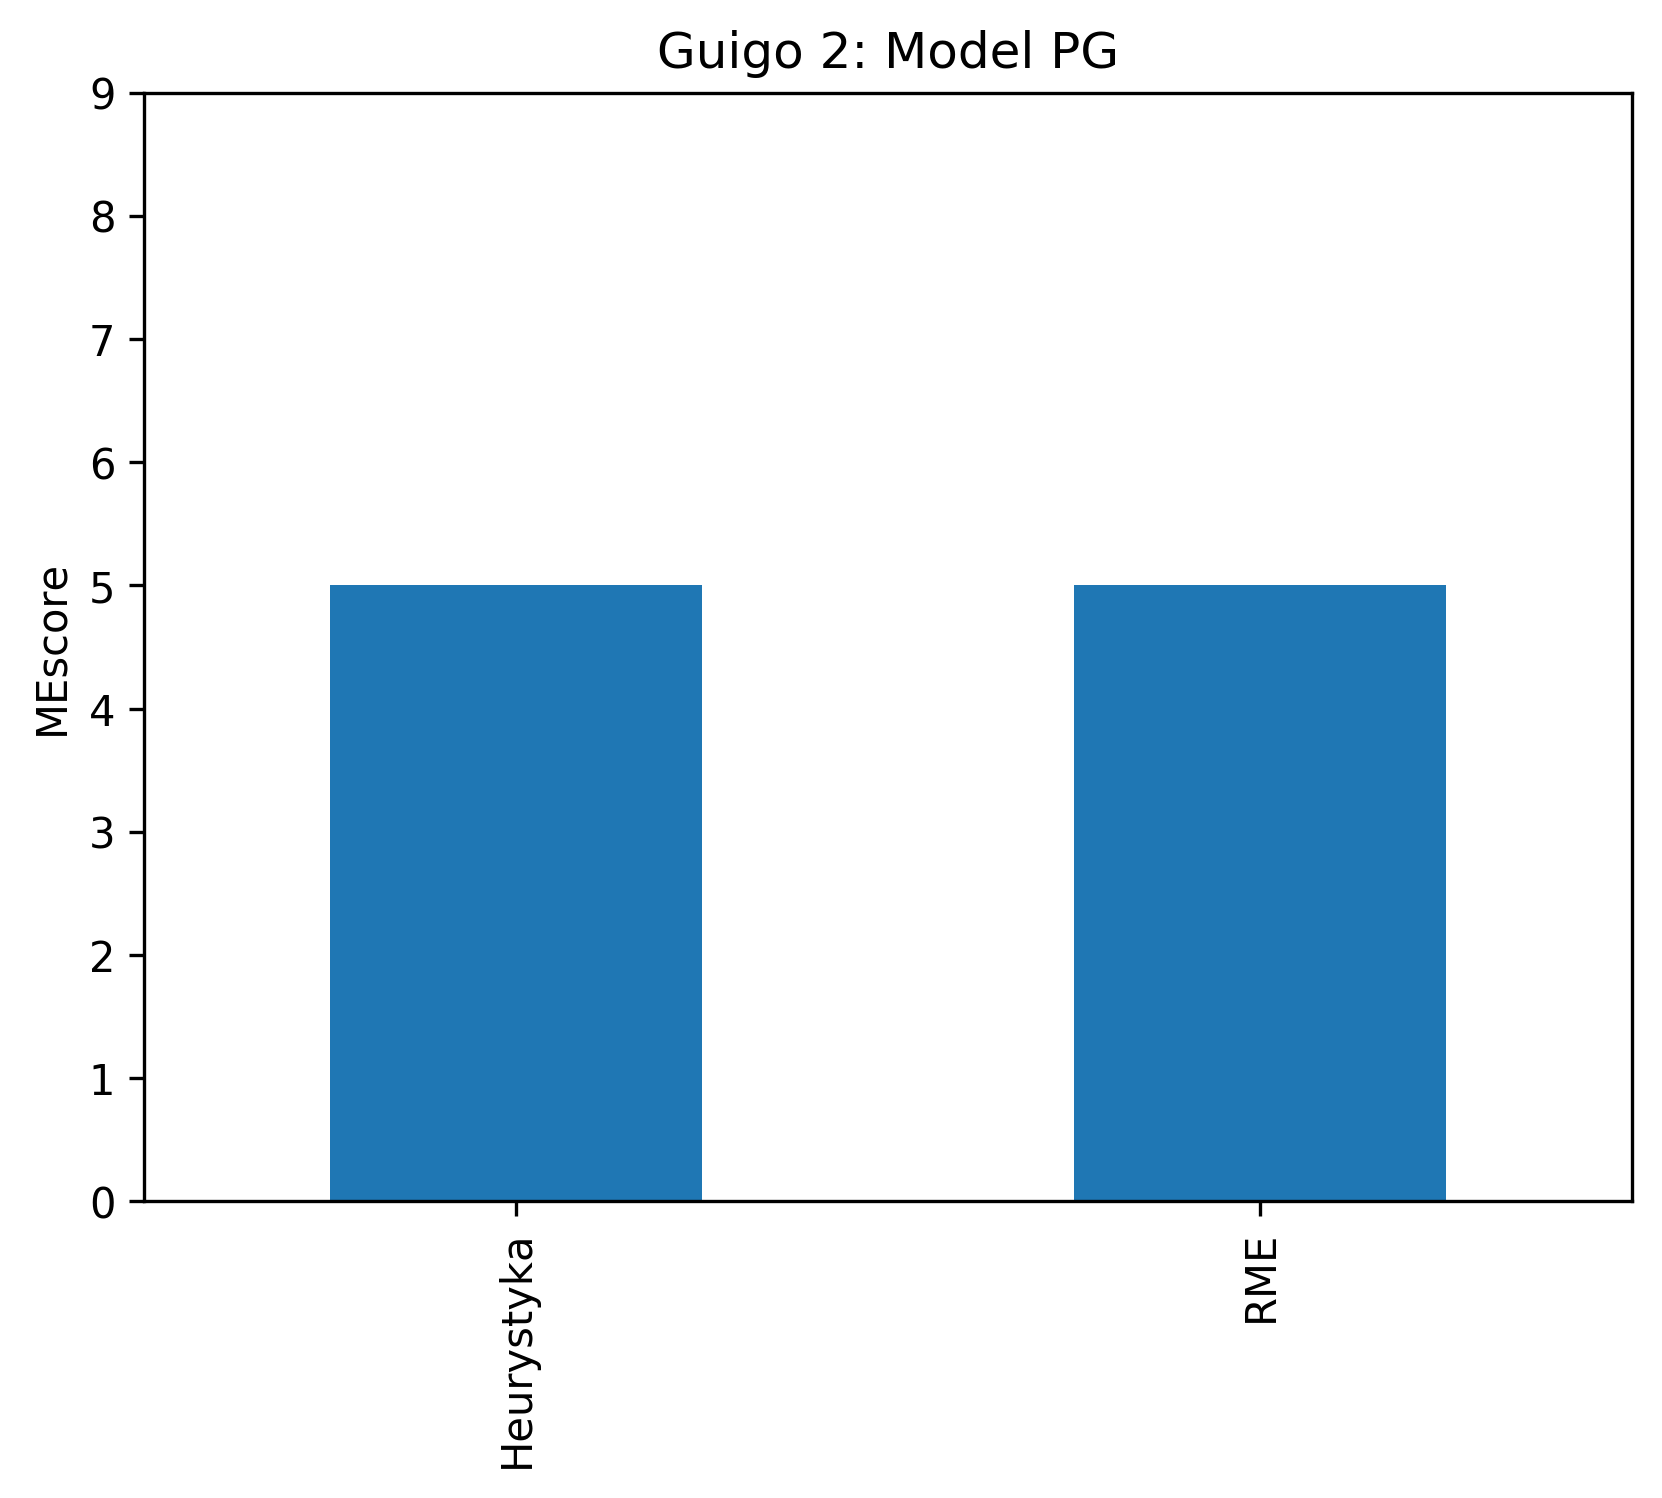
\includegraphics[width=50mm]{./pictures/G2_PG.png}
  \caption{Test algorytmu dla modelu PG}
\end{subfigure}%
\begin{subfigure}{.5\textwidth}
  \centering
  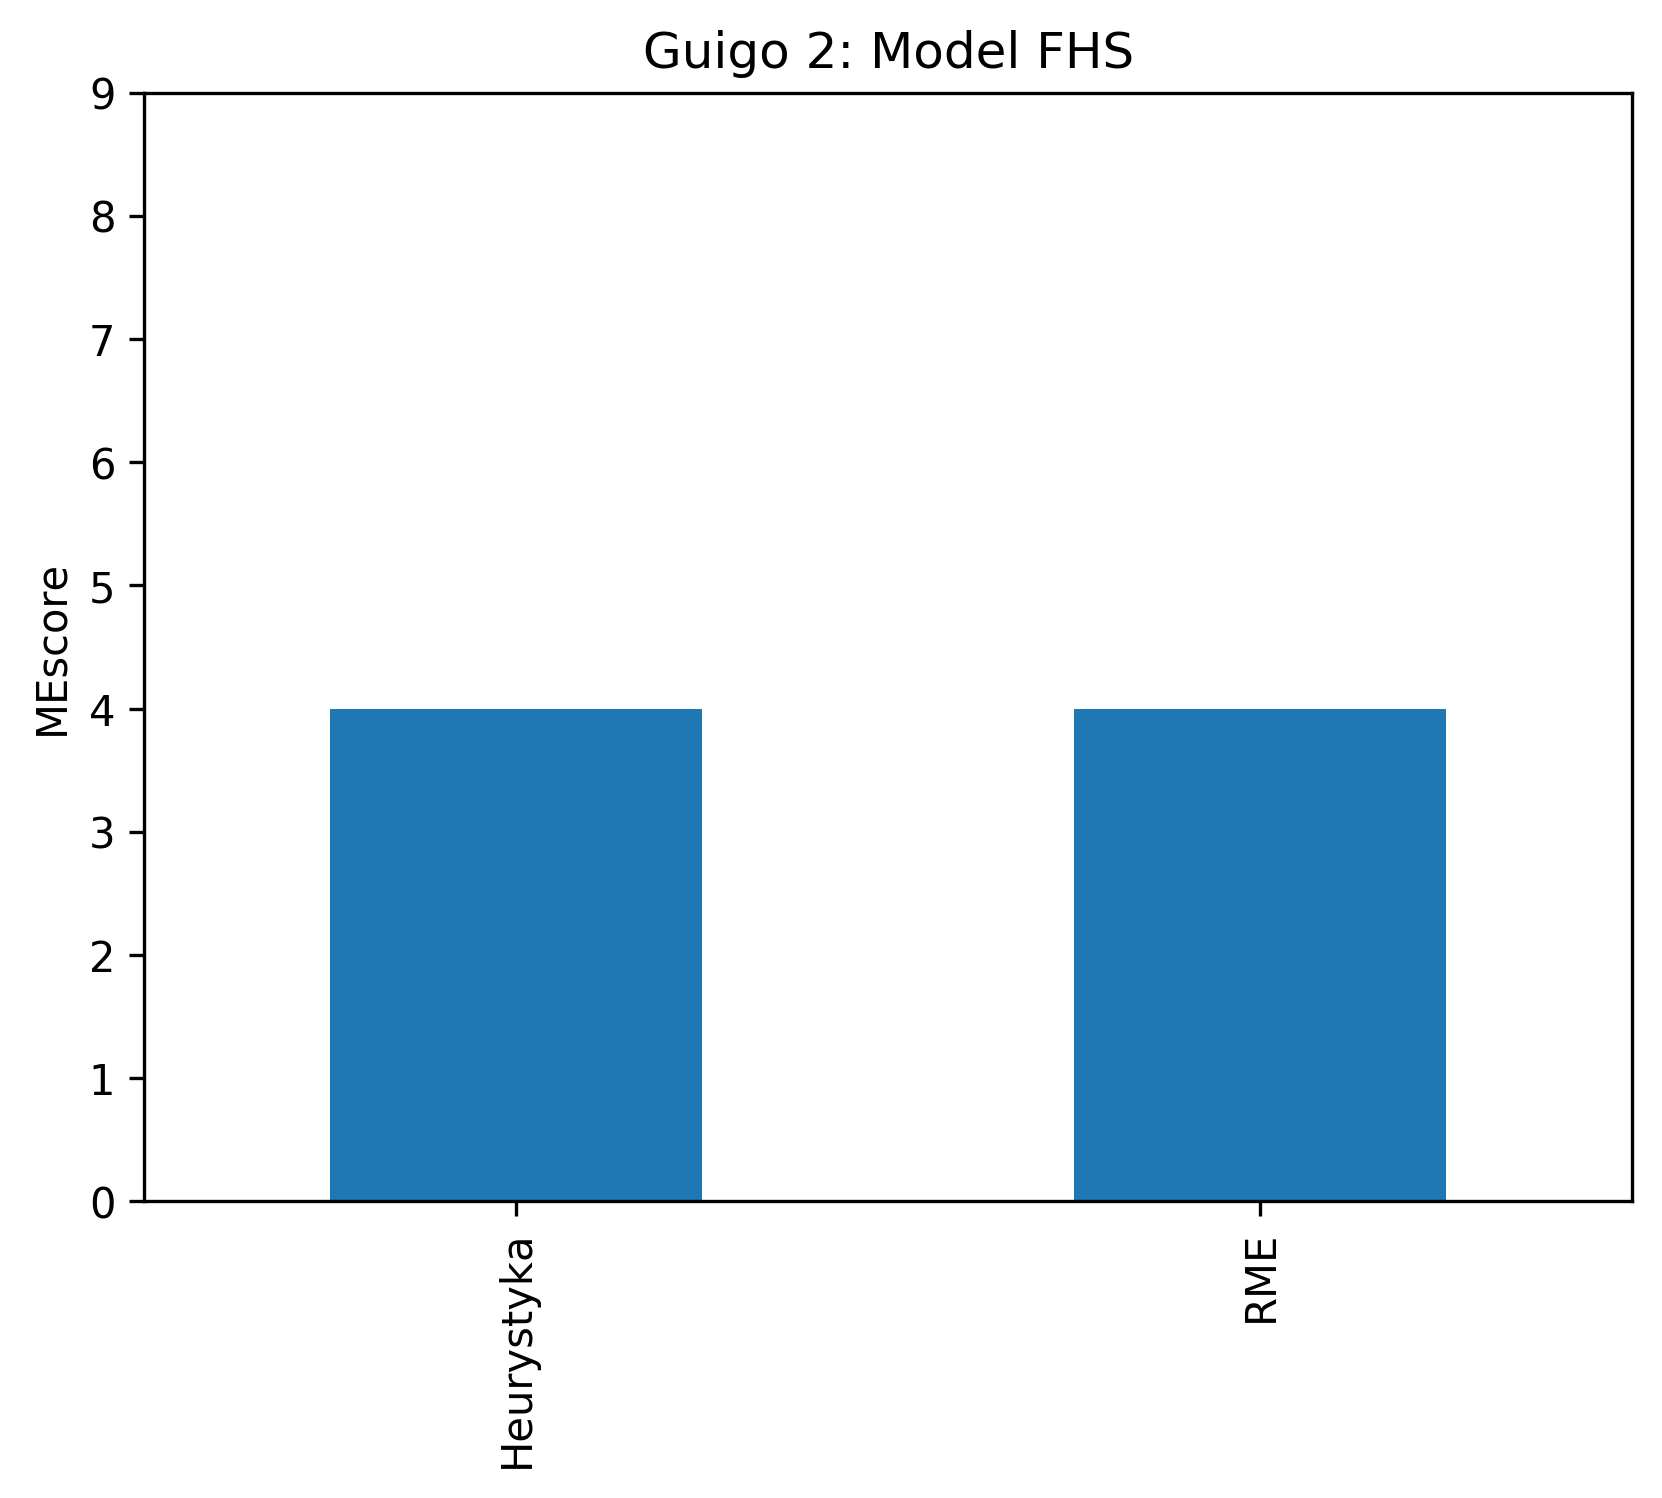
\includegraphics[width=50mm]{./pictures/G2_FHS.png}
  \caption{Test algorytmu dla modelu FHS}
\end{subfigure}%
\caption{Testy algorytmu na danych rzeczywistych dla drzewa gatunków $S_2$}
\end{figure}

Dla wszystkich przypadków algorytm jest w stanie osiągnąć wyniki identyczne jak te wyliczone przez program RME. 

\subsection{Testy algorytmu na danych symulowanych}
Dane dla testów syntetycznych zostały wygenerowany w sposób losowy jednak wielkość, struktura i ilość drzew genów zostały dopasowane do zbioru Guigo. Zbiory symulowane zawierają syntetyczne drzewo gatunków z 15 liśćmi wygenerowane z modelu Yule'a \cite{pmid11259805} oraz 48 ukorzenionych drzew genów etykietowane gatunkami z wylosowanego wcześniej drzewa gatunków. Przykładowe drzewa gatunków (w formie graficznej) i genów (w formie tekstowej) można znaleźć w dodatkach do pracy. Test został przeprowadzony dla 10000 losowych zestawów.

\begin{figure}[H]
\centering
\begin{subfigure}{.5\textwidth}
  \centering
  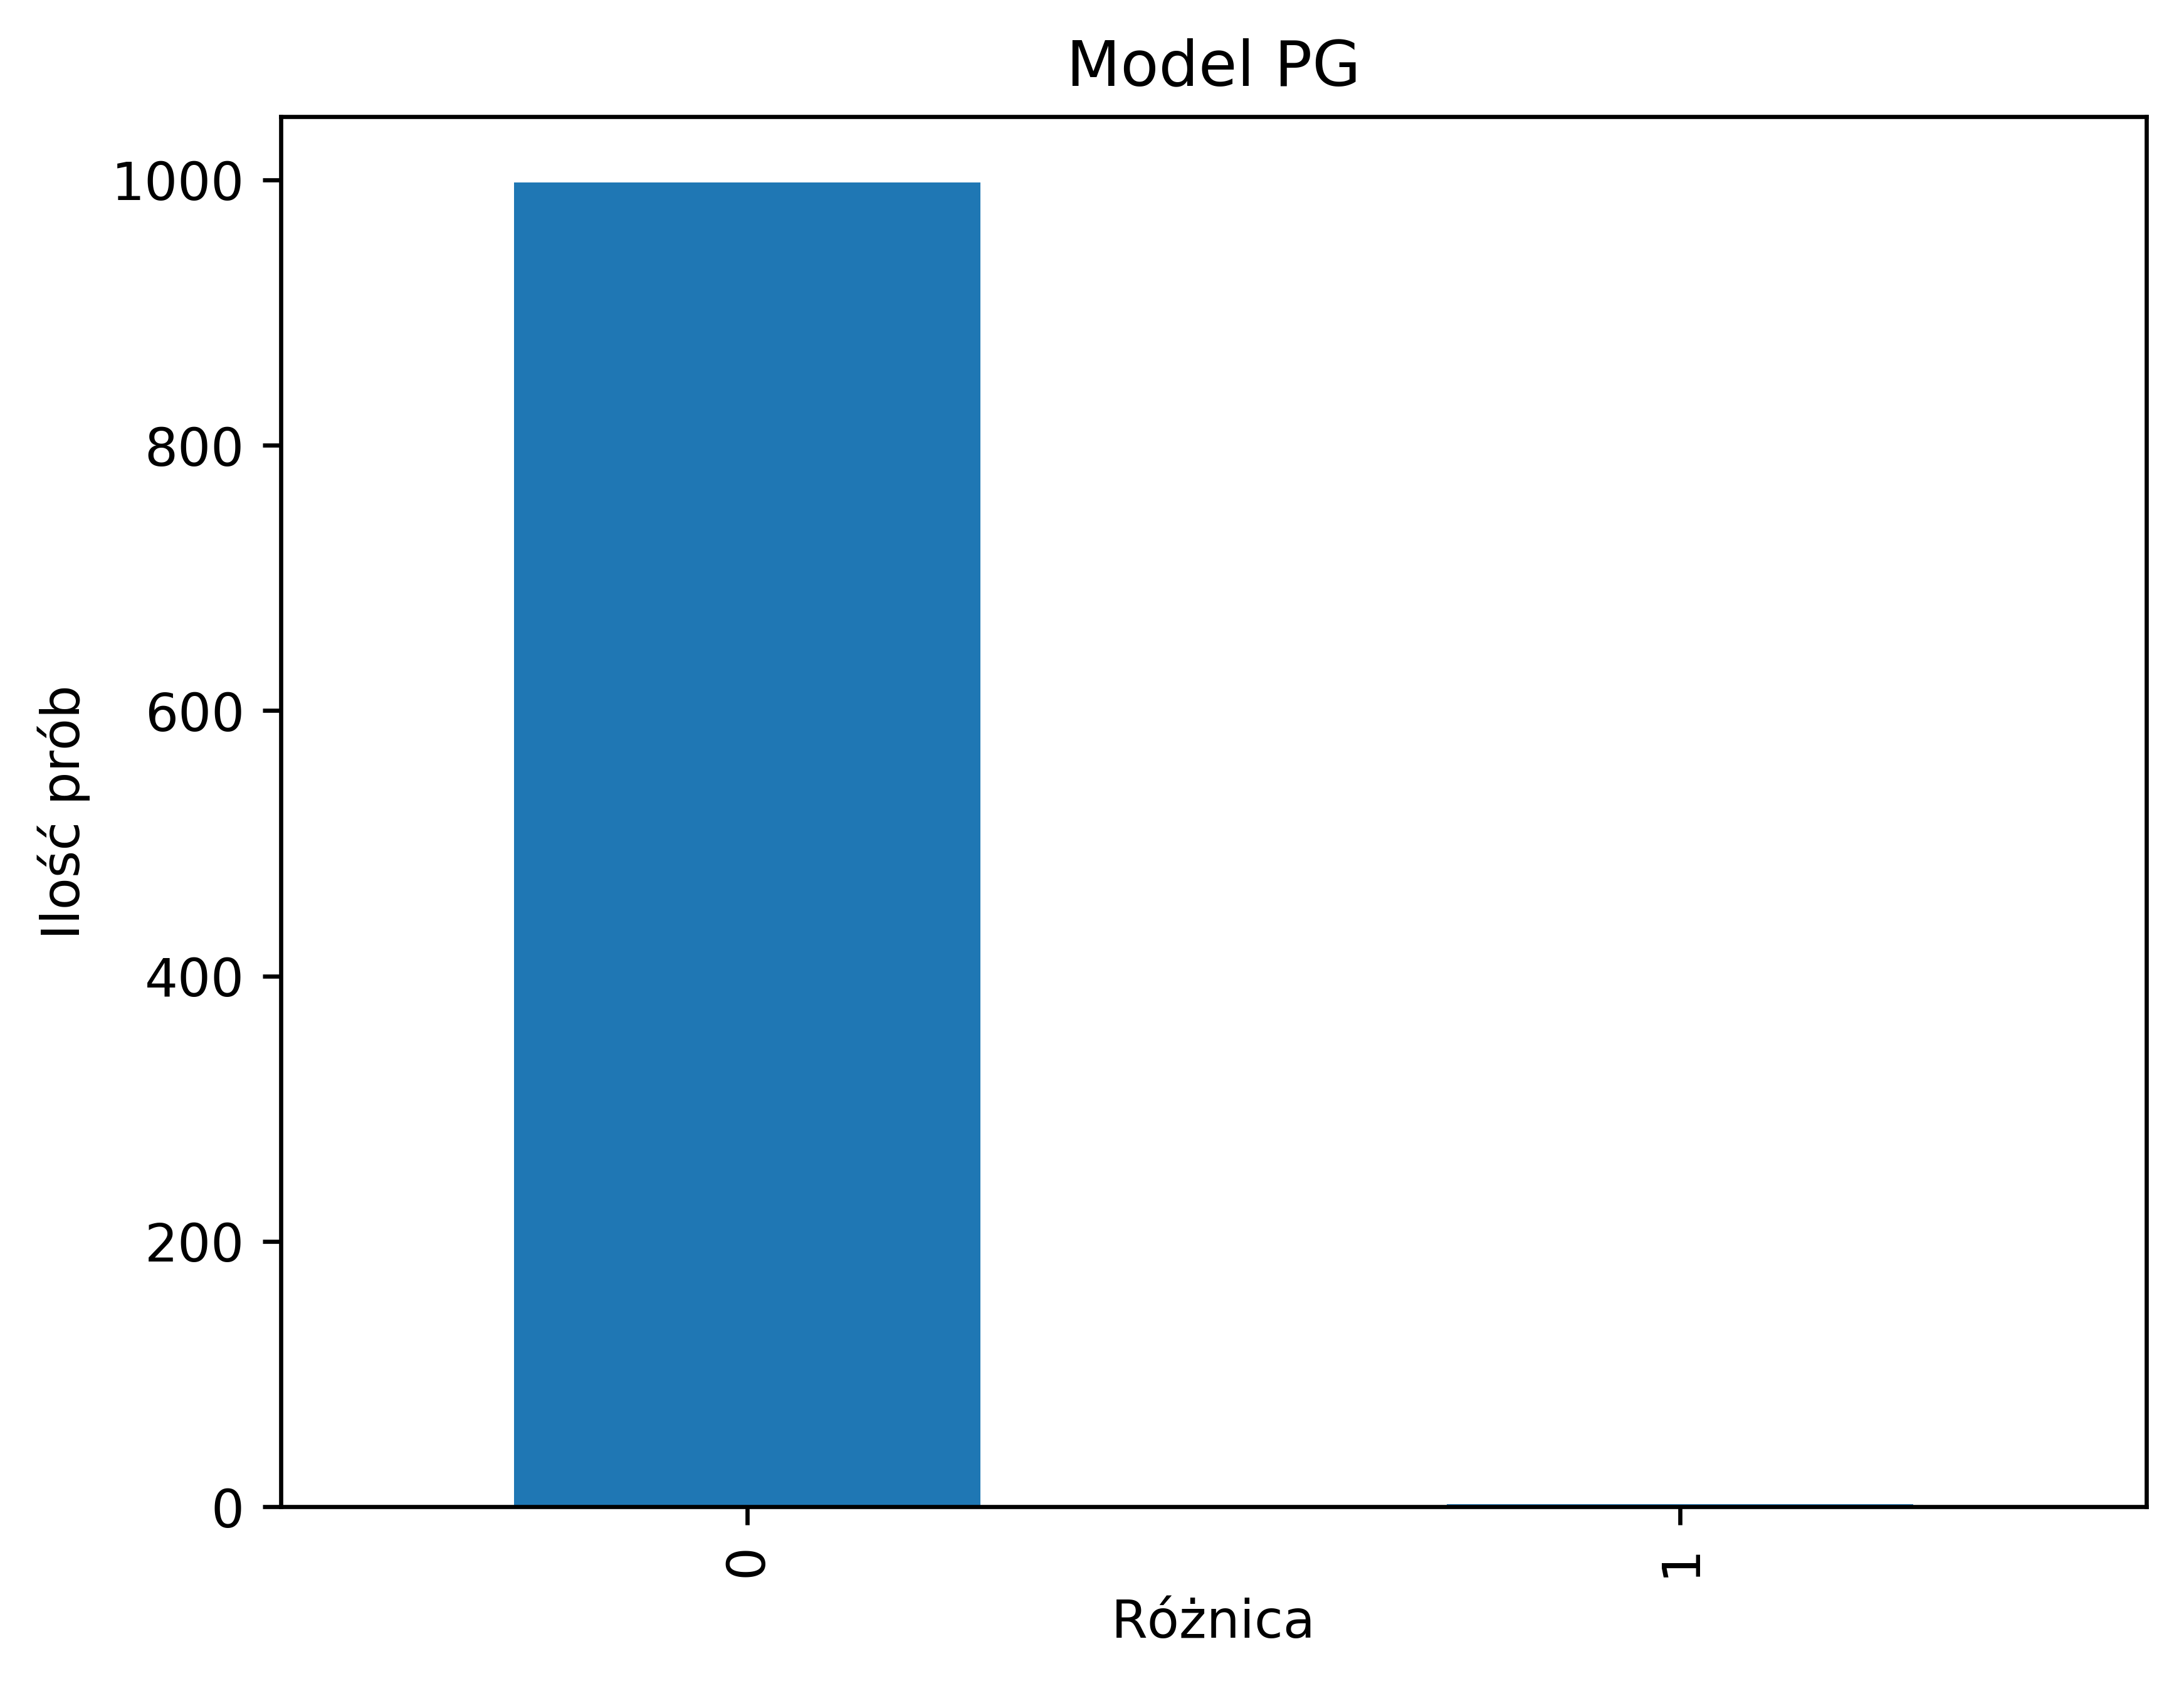
\includegraphics[width=50mm]{./pictures/PG.png}
  \caption{Test algorytmu dla modelu PG}
\end{subfigure}%
\begin{subfigure}{.5\textwidth}
  \centering
  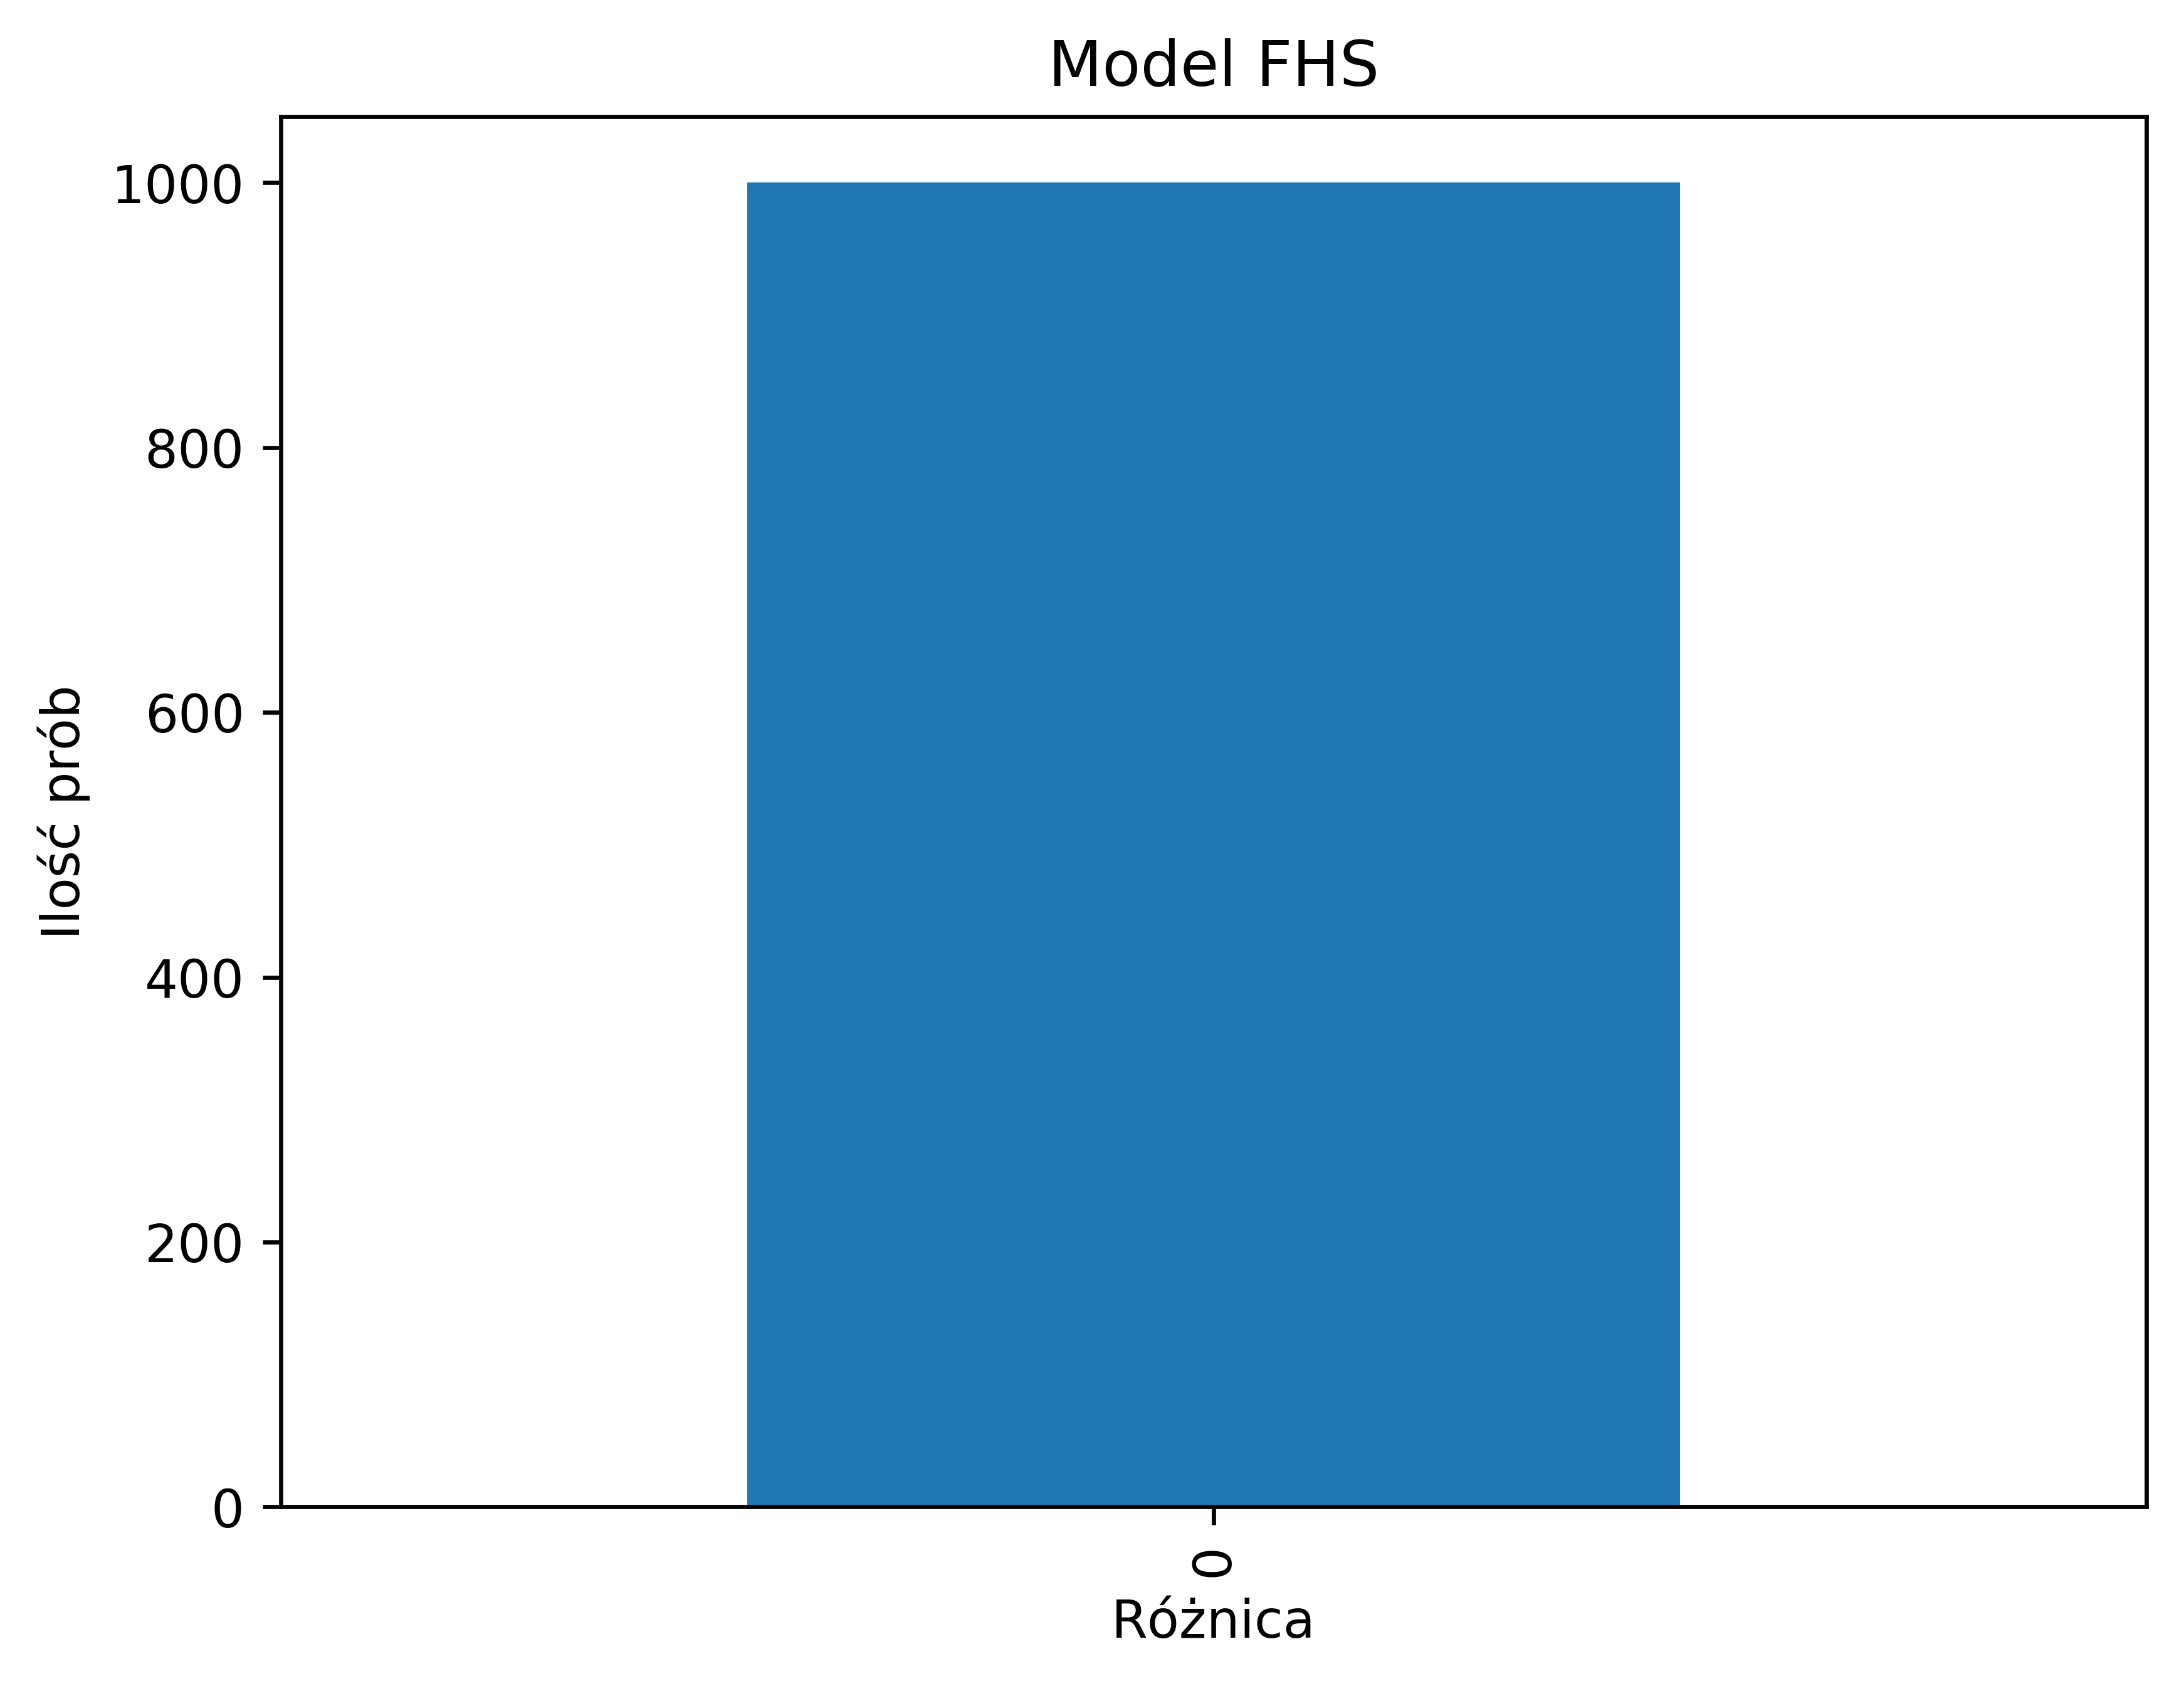
\includegraphics[width=50mm]{./pictures/FHS.png}
  \caption{Test algorytmu dla modelu FHS}
\end{subfigure}%
\caption{Testy algorytmu na danych symulowanych. Przez różnicę rozumiany jest wynik odjęcia od wyliczeń otrzymanych przez program RME wyliczeń otrzymanych dzięki proponowanemu algorytmowi. }
\end{figure}

W obu przypadkach wyniki obliczeń heurystyki nie odbiegają od wartości kosztu ewolucyjnego otrzymanych przez program RME i dla wszystkich przypadków algorytm jest w stanie osiągnąć identyczny wynik.

\chapter{Podsumowanie}

W~pracy przedstawiono pierwszy pomysł na ocenę scenariuszy ewolucyjnych reprezentowanymi drzewami DLS pod kątem liczby duplikacji. Należy jednak wspomnieć, że samą ideę da się znacząco usprawnić. 
\\
Obecnie to krok w którym konieczne jest wyliczenie zbioru drzew semi-normalnych dla danego drzewa genów jest krokiem najbardziej wymagającym czasowo i obliczeniowo. Nie udało się jednak zaobserwować, by zaimplementowany algorytm kiedykolwiek potrzebował więcej niż jedną sekundę na wczytanie danych i więcej niż 0.3 sekundy na obliczenie drzewa o najmniejszym koszcie ewolucyjnym. Jest to dużo lepszy wynik od programu RME, który dla modelu FHS, potrzebował nawet kilkunastu sekund na wyliczenie minimalnego kosztu duplikacujnego. 
Należy jednak podkreślić, że to właśnie program DLSgen był swego rodzaju "wąskim gardłem"~i~niemożliwe jest przetestowanie algorytmu na danych bardziej złożonych niż zbiór Guigo lub jego pochodne. 
\\
Testy pokazują również, że opisany algorytm zwraca wyniki, które nie różnią się od rzeczywistego minimalnego kosztu ewolucyjnego, gdyż dla wszystkich przypadków uzyskano najniższe możliwe wyniki. Może to jednak wynikać z dosyć niskiego kosztu duplikacyjnego wyliczonego przez oba programy. Wynosił on maksymalnie 11 (średnia arytmetyczna = 6.1, mediana = 6 ) dla modelu PG i 7 (średnia arytmetyczna = 4.5, mediana = 4) dla modelu FHS. Proponowany algorytm wymaga w związku z tym kolejnych, bardziej rozbudowanych testów.


\section{Perspektywy rozwoju}

Trudno przewidzieć wszystkie możliwości rozwoju algorytmu, ale tę bardziej
oczywistą można wskazać już teraz.  Jest to uniezależnienie algorytmu od kroku w którym wyliczane są scenariusze i klastrowanie duplikacji bezpośrednio na podstawie drzew genów. Jest to krok kluczowy dla dalszego rozwoju heurystyki, ponieważ pozwoli on na używanie jej przy rozwiązywaniu rzeczywistych problemów. Będzie możliwe wtedy również przeprowadzenie testów dla danych dużo bardziej skomplikowanych i bardziej przystających do obecnych problemów niż zbiór Guigo.

\section{Perspektywy wykorzystania}

Podstawową zaletą przedstawionej heurystyki jest jej uniwersalność. Ocena scenariuszy nie zależy od obranego modelu, a obecnie wydaje się, że same obliczenia nie są obarczone błędem. Kolejną niewątpliwą zaletą jest fakt, że w istocie również struktura drzewa nie ma dla algorytmu dużego znaczenia. Drzewo binarne nie zawsze jest najlepszym przedstawieniem historii ewolucji i algorytm jest na taką zmianę gotowy. Z punktu widzenia heurystyki drzewa są tablicą zawierającą liczbę klastrów duplikacyjnych dla danego węzła w drzewie gatunków, a które umieszczone są w niej w porządku prefiksowym. Zapewnia to możliwość wykorzystania algorytmu nie tylko dla drzew binarnych. Pokreślić trzeba jednak, że obecnie algorytm istnieje w formie prototypowej i wymaga wzmożonej oraz dokładnej pracy.  

\appendix

\chapter{Pętla programu zapisana w~języku Python wykonywana dla losowego wybierania indeksów}

\begin{verbatim}

		max_trees = []
        for scenario in self:
            all_dup_pref = [tree.duplication_prefix for tree n scenario]
            max_trees.append(self.rate_scenario(all_dup_pref))
        max_tree = self.rate_scenario(max_trees)

        if select_type == "random":

            index_list = [x for x in range(len(max_tree)) if x != 0]

            while index_list:
                index_list_position = random.randint(0, len(index_list) - 1)
                index = index_list[index_list_position]

                max_tree_temp = max_tree[:]
                max_tree_temp[index] -= 1

                for scenario in self:
                    for tree in scenario:
                        for i in range(len(tree.duplication_prefix)):
                            if max_tree_temp[i] - tree.duplication_prefix[i] < 0:
                                break
                        else:
                            break
                    else:
                        index_list.pop(index_list_position)
                        break
                else:
                    max_tree = max_tree_temp
            return max_tree, sum(max_tree)
\end{verbatim}

\chapter{Przykładowe drzewa gatunków dla danych syntetycznych}



\begin{figure}[H]
  \centering
  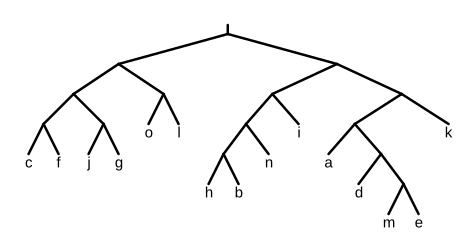
\includegraphics[width=80mm]{./pictures/syn_spec_1.png}
  \caption{Drzewo gatunków $S_1$}
\end{figure}

\begin{figure}[H]
  \centering
  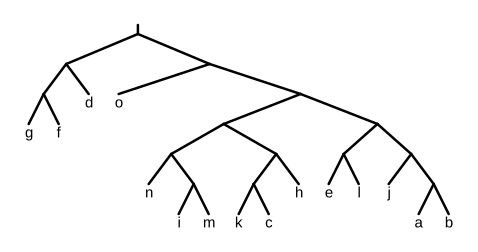
\includegraphics[width=80mm]{./pictures/syn_spec_2.png}
  \caption{Drzewo gatunków $S_2$}
\end{figure}


\chapter{Przykładowe drzewa genów dla danych syntetycznych}
\begin{obeylines}
Format tekstowy:
((b,l),h)
((a,k),b)
((i,k),a)
((l,b),o)
(h,(j,o))
(b,(i,c))
(b,(m,j))
((m,a),b)
((g,m),f)
((a,l),k)
(o,(j,h))
((k,d),i)
(e,(c,o))
(f,(a,h))
(j,(k,d))
((k,e),c)
(j,(e,b))
((i,n),l)
(f,(b,h))
(c,(k,g))
((l,o),j)
((a,f),d)
((f,h),j)
(h,(d,n))
((b,j),i)
((a,e),(g,l))
((b,c),(n,o))
(m,((j,h),d))
((e,(f,g)),a)
(((m,d),g),a)
((h,l),(n,b))
((d,(b,a)),k)
(((k,n),c),m)
(((d,c),b),(j,a))
(c,((l,(g,j)),k))
(((h,g),(a,e)),l)
((o,(f,e)),(j,h))
((g,l),((c,m),n))
((e,(f,(j,o))),k)
(f,(a,((n,h),(b,c))))
((a,(o,h)),((e,i),n))
((e,d),((a,b),(n,g)))
(((m,(d,b)),j),(f,e))
((l,h),(((a,j),((m,g),f)),e))
((n,(i,e)),(((a,k),f),(l,b)))
((j,e),(i,((a,(k,(l,d))),n)))
((((f,k),(b,(o,e))),((g,n),j)),m)
(h,((b,(m,f)),((c,j),(a,(k,l)))))
\end{obeylines}

\newpage
\addcontentsline{toc}{chapter}{Bibliografia}
\bibliography{dup_claster.bib}
\bibliographystyle{nar}
\end{document}


%%% Local Variables:
%%% mode: latex
%%% TeX-master: t
%%% coding: latin-2
%%% End:
